\documentclass[handout]{beamer}
\usetheme[secheader]{Boadilla}

\usepackage{tikz}
\usetikzlibrary{shapes.callouts}

\mode<presentation>{}

\usepackage{boxedminipage}
\usepackage{pgf}
\usepackage{graphicx}
\usepackage{amsmath}
\usepackage{amssymb,amsmath,amsthm}
\usepackage{colortbl}
\usepackage{xspace}
\usepackage{xcolor}

\usepackage{amssymb,amsmath,amsthm}
\usepackage{boxedminipage}

\beamerboxesdeclarecolorscheme{monscheme}{structure}{gray!25}
\beamertemplatetransparentcovereddynamic


\colorlet{myblue}{blue!80!black}
\colorlet{mygreen}{green!80!black}

\newcommand{\from}{\leftarrow}
\newcommand{\ignore}[1]{}
\newcommand{\algofont}[1]{{\mathsf{#1}}}
\newcommand{\gamefont}[1]{{\mathsf{#1}}}
\newcommand{\objfont}[1]{{\mathtt{#1}}}
\newcommand{\secprm}{\lambda}

\newcommand{\calA}{\mathcal{A}}
\newcommand{\calD}{\mathcal{D}}
\newcommand{\calF}{\mathcal{F}}
\newcommand{\st}{\mathtt{st}}


\newcommand{\anamorphicPrefix}{\algofont{a}}
\newcommand{\anamorphicPrefixObj}{\objfont{a}}
\newcommand{\ame}{\algofont{AME}}
\newcommand{\akg}{\anamorphicPrefix\kg} 
\newcommand{\aenc}{\anamorphicPrefix\enc}
\newcommand{\adec}{\anamorphicPrefix\dec}
\newcommand{\apk}{\anamorphicPrefixObj\pk}
\newcommand{\ask}{\anamorphicPrefixObj\sk}
\newcommand{\dkey}{\objfont{dkey}}
\newcommand{\act}{\anamorphicPrefixObj\ct}
\newcommand{\amsg}{\anamorphicPrefixObj\msg}


%%anamorphic games
\newcommand{\RealG}{\gamefont{RealG}}             %real
\newcommand{\AnamorphicG}{\gamefont{AnamorphicG}} %anamorphic 
\newcommand{\Oa}{\algofont{Oa}}
\newcommand{\Oe}{\algofont{Oe}}

%algorithms for encryption schemes
%\newcommand{\encryptionSchemeName}{\calE}
\newcommand{\E}{\algofont{E}}
\newcommand{\kg}{\algofont{KG}}
\newcommand{\enc}{\algofont{Enc}}
\newcommand{\dec}{\algofont{Dec}}
%objects of encryption schemes
\newcommand{\pk}{\objfont{pk}}      %public key
\newcommand{\sk}{\objfont{sk}}      %secret key
\newcommand{\msg}{\objfont{msg}}    %cleartext
\newcommand{\ct}{\objfont{ct}}      %ciphertext

%encryption scheme with pseudoR ciphertexts
\newcommand{\prPrefix}{\algofont{pr}}
\newcommand{\prObjPrefix}{\objfont{pr}}
\newcommand{\prEname}{\prPrefix\E}
\newcommand{\prkg}{\prPrefix\kg}
\newcommand{\prenc}{\prPrefix\enc}
\newcommand{\prdec}{\prPrefix\dec}
\newcommand{\prct}{\prObjPrefix\ct}
\newcommand{\prkey}{\prObjPrefix\objfont{K}}


\newcommand{\rrdec}{\algofont{rr}\dec}


\newcommand{\PameG}{\gamefont{SingleAnG}}        %private anamorphic --> single



\title[Anamorphic]{Anamorphic Encryption}
\subtitle{Private Communication against a Dictator}
%\title[Short Title]{Long Title}

\author{Giuseppe Persiano, Duong Hieu Phan, Moti Yung}
\date{}

\begin{document}

\begin{frame}
  \titlepage


Eurocrypt 2022 -- Trondheim 
\end{frame}


\begin{frame}
\frametitle{Privacy as a Human Right}

UDHR, Article 12: (1948)

{\color{brown}
{\em No one shall be subjected to arbitrary interference with his privacy, family, home or correspondence,...}
}

\pause
\vskip 1cm
\begin{block}{End to End Encryption}
\begin{itemize}
\item Cryptography has been very successful in providing tools for
encrypting communication
\begin{itemize}
\item The Signal protocol and app \hfill 
\includegraphics[width=.5cm]{imgs/signal}
\end{itemize}
\end{itemize}
\end{block}

\pause
\vfill
But its success relies on two assumptions that might be challenged in dictatorial
states
\end{frame}

\begin{frame}
\frametitle{The receiver-privacy assumption}

{\color{brown} \em 
Encryption guarantees message confidentiality only with respect to 
parties that do not have access to  the receiver's private key
}

\vfill


\begin{block}{The receiver-privacy assumption}
The receiver keeps his secret key in a private location
\end{block}

\end{frame}

\begin{frame}
\frametitle{The sender-freedom assumption}

{\color{brown} \em 
A ciphertext carries the message that was provided as an input,
not the one that the sender wishes to encrypt
}

\vfill

\begin{block}{The sender-freedom assumption}
The sender is free to pick the message to be encrypted
\end{block}
\end{frame}

\begin{frame}
\frametitle{Ok...two more assumptions}

Why is this a problem?

\begin{theorem}
Assume 
{\color{brown} existence of one-way functions} 
and 
{\color{brown} receiver privacy}.
Then, there exist secure symmetric encryption schemes.
\end{theorem}

\vfill
\begin{block}{Two assumptions}
\begin{itemize}
\item Existence of one-way functions
\item Ability to hide my key
\end{itemize}
\end{block}
\end{frame}

\begin{frame}
\frametitle{Law of Nature vs Normative Prescription}

\begin{itemize}
\item {\color{green} Assumption of the existence of one-way functions comes from
{\em our current scientific understanding of Nature}}
 
    \begin{itemize}
        \item {\color{blue}if true, it is enforced by Nature}
        \item {\color{blue}it might be false but then it is false for all}
    \end{itemize}
\vskip 1cm
\item {\color{green} Receiver privacy is a {\em norm}: }
    
    \begin{itemize}
        \item {\color{blue} it is enforced by political power}
        \item {\color{blue} it can be changed by law, decree, force}
        \item {\color{blue} it could change for some but not for all}
    \end{itemize}
\end{itemize}

\end{frame}

\begin{frame}
\frametitle{Receiver privacy and Sender freedom}
\begin{itemize}
\item Both assumptions are realistic for ``{\color{purple} normal}'' settings
\item No wonder Encryption has been developed under these assumptions
\begin{itemize}
\item with no explicit mention
\end{itemize}
\pause
\vskip .5cm
\item In a dictatorship, instead
\pause
\begin{itemize}
\item {\color{blue} No receiver privacy:} 
citizens might be invited to surrender their private keys

\centerline{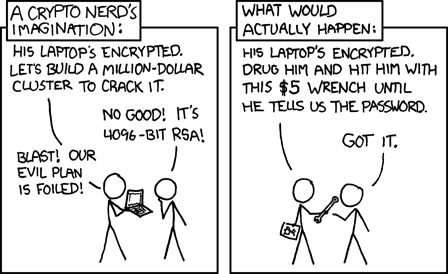
\includegraphics[width=4.1cm]{imgs/xkcd}}

\item {\color{blue} No sender freedom:} 
citizens might be invited to send messages to international newspapers
to make the dictator look good
\end{itemize}
\end{itemize}
\end{frame}


\begin{frame}
\frametitle{Not only dictators...}

Various attempts to regulate, limit, cripple encryption
\begin{block}{Crypto Wars}
{\em\color{brown} Presently, anyone can obtain encryption devices for voice or data transmissions. [...]
if criminals can use advanced encryption technology in
their transmissions, electronic surveillance techniques could be rendered 
useless because of law enforcement’s inability to decode the message.}

\medskip

\hfill {\color{brown} Howard S. Dakoff}

\hfill {\color{brown} {\em The Clipper Chip Proposal}}

\hfill {\color{brown} J. Marshall L. Rev., 29, 1996.}
\end{block}

\end{frame}

\begin{frame}
\frametitle{Crypto Wars}

\begin{itemize}
\item Combination of cryptographic tools and normative prescription

\item From [Micali 1992] to [Green-Kaptchuk-van Laer 2021]

\begin{itemize}
\item Rely on the existence of an independent judiciary system (missing in a Dictatorship!)
\end{itemize}
\item Kleptography [Young-Yung 97]
\item Subvertable encryption
\end{itemize}
\end{frame}


\ignore{
\begin{frame}
\frametitle{How can we fix it?}

\begin{block}{A new research problem}
{\em Design new encryption schemes that can be proved secure
without relying on the receiver-privacy assumption}
\end{block}

\vskip 1cm
\begin{block}{Another new research problem}
{\em Design new encryption schemes that can be proved secure
without relying on the sender-freedom assumption}
\end{block}
\pause

{\tikz[remember picture,overlay]{
        \node[inner sep=10pt,ellipse callout,shading=ball,]at(8,6.4)[white]{
            What does it mean?};}}
\end{frame}
}
\begin{frame}
\frametitle{How can we fix this?}

{\color{blue} Not by designing new schemes}

\pause

\begin{itemize}
\item Suppose we design an encryption scheme that is secure 
without assuming receiver privacy and/or sender freedom

\item What is the dictator going to do?

    \begin{itemize}
    \item It will be considered illegal
    \item The simple act of using the new scheme will be self accusatory
    \item The encryption scheme and its use will be seen as provocations
    \end{itemize}

\end{itemize}

\pause

\vskip 1cm
{\color{brown}\em 
Rather, we should look at {\em existing} schemes to see if they can
be used to defeat the dictator
}

\pause

\vfill
Existing schemes cannot be disallowed as there are legitimate uses for
them. Legitimate, even for the dictator.
\end{frame}

\begin{frame}
\frametitle{Our approach}
Let us focus first on receiver privacy
\pause
\begin{block}{Constraints}
\begin{itemize}
\item If the dictator has the secret key $\color{blue} \mathtt{sk}$,
        it can decrypt and read the message.

\item But only the message encrypted with respect to $\color{blue} \mathtt{sk}$ can be decrypted.
\end{itemize}
\end{block}

\pause
\vfill

\begin{block}{Our approach}
\begin{itemize}
\item A ciphertext is associated with {\color{purple} two} secret keys 
$\color{blue} \mathtt{sk_0,sk_1}$
\item A ciphertext carries two plaintexts $\color{blue} m_0,m_1$,
one for each key
\item {\color{brown} ...and there is {\bf no} second key}
    \begin{itemize}
        \item at least, that's what the dictator thinks
    \end{itemize}
\end{itemize}
\end{block}

\end{frame}

\begin{frame}
\frametitle{Rejection Sampling Encryption}
\hfill Bellare, Paterson, Rogaway [CRYPTO14]

\hfill Horel, Park, Richelson, Vaikuntanathan [ITCS19]
\begin{block}{Normal mode}
\begin{itemize}
\item $\color{blue}\calE=(\kg,\enc,\dec)$ any encryption scheme
\item Alice has $\color{blue}(\pk,\sk)$
\item Bob computes $\color{blue}\ct=\enc(\pk,\text{\color{purple} ``Glory to our Leader''})$
\item Dictator decrypts $\color{blue}\ct$ using $\color{blue}\sk$
\end{itemize}
\end{block}

\pause

\begin{block}{Anamorphic mode}
\begin{itemize}
\item Alice and Bob share a randomly chosen seed $\color{blue} K$ for a PRF
$\color{blue}\calF$
\item Bob wants to send a bit $\color{blue} b$ to Alice 

    \begin{itemize}
        \item samples $\color{blue}\ct=\enc(\pk,\text{\color{purple} ``Glory to our Leader''})$
        \item until $\color{blue}\calF(K,\ct)=b$
    \end{itemize}

\end{itemize}
\end{block}
\end{frame}

\ignore{
\begin{frame}
\begin{block}{Our approach}
\begin{itemize}
\only<1->{
\item A ciphertext is associated with {\color{purple} two} secret keys 
$\color{blue} \mathtt{sk_0,sk_1}$
}

\only<2->{$$\color{blue} \sk_0:=\sk \qquad \sk_1:=K$$}

\only<3->{\item A ciphertext carries two plaintexts $\color{blue} m_0,m_1$, 
one for each key}

\only<4->{$$\color{blue} m_0:=\text{\color{purple}``Glory to our Leader''} \qquad m_1:=b$$}

\only<5->{\item {\color{brown} ...and there is {\bf no} second key}}
    \only<6->{\begin{itemize}
        \item $\color{blue}\calE$ is just an off-the-shelf encryption scheme
        \item no need for $\color{blue}K$
    \end{itemize}
    }
\end{itemize}
\end{block}
\end{frame}
}

\begin{frame}
\frametitle{Receiver privacy}

\begin{block}{Feasibility result}
{\color{brown} 
Rejection sampling encryption gives a one-bit symmetric
encryption scheme whose secure does not rely on the receiver-privacy
assumption.
}

\end{block}

\pause
\vfill
\begin{block}{Rate}

\begin{itemize}
\item {\em \color{brown} Rejection Sampling} can be extended to any length $\ell$ 
\item Average encryption time is exponential in $\ell$
\end{itemize}
\end{block}
\pause
\vfill
{\color{purple} Receiver Anamorphic}
\end{frame}

\begin{frame}
\frametitle{Our technical contribution}

\begin{itemize}
\item  {\color{purple} Receiver Anamorphic} for many bits
    \begin{itemize}
        \item Rejection Sampling only work for few bits
    \end{itemize}
    \vskip 2cm
\item  {\color{purple} Sender Anamorphic} with no shared key
    \begin{itemize}
        \item Rejection Sampling assumes Alice and Bob share a key
    \end{itemize}
    for this we need extra properties 
\end{itemize}
\end{frame}

\begin{frame}
\frametitle{The Naor-Yung Encryption Scheme}
\begin{exampleblock}{Normal Mode}
\begin{itemize}
\item Let $\color{blue}\calE=(\kg,\enc,\dec)$ any encryption scheme
\item Alice runs $\color{blue} \kg$ twice, randomly selects $\color{blue} \Sigma$ 
and sets $\color{blue} \pk=(\pk_0,\pk_1,\Sigma)$ and $\color{blue} \sk=\sk_0$
\item If Bob wants to send {\color{purple} ``Glory to our Leader''} to Alice
    \begin{itemize}
    \item Compute $\color{blue} \ct_0=\enc(\pk_0,\text{\color{purple} ``Glory to our Leader''})$
    \item Compute $\color{blue} \ct_1=\enc(\pk_1,\text{\color{purple} ``Glory to our Leader''})$
    \item Compute NIZK proof $\color{blue} \Pi$ that $\color{blue} \ct_0$ and $\color{blue} \ct_1$ carry the same    
        plaintext
    \item Set $\color{blue} \ct=(\ct_0,\ct_1,\Pi)$
    \end{itemize}
\item To decrypt $\color{blue} \ct$, Alice
    \begin{itemize}
        \item Checks $\color{blue} \Pi$ is a valid proof
        \item If valid decrypts $\color{blue} \ct_0$ using $\color{blue} \sk$
    \end{itemize}
\end{itemize}
\end{exampleblock}
\end{frame}

\begin{frame}
\frametitle{The Naor-Yung Encryption Scheme}
\begin{exampleblock}{Anamorphic Mode}
\begin{itemize}
\item Alice runs $\color{blue} \kg$ twice, runs the simulator to get $\color{blue}(\Sigma,\mathtt{aux})$ 
and sets $\color{blue} \pk=(\pk_0,\pk_1,\Sigma)$ and $\color{blue} \sk=(\sk_0,\sk_1)$
\item $\color{blue}\mathtt{aux}$ is shared with Bob
\item If Bob wants to send {\color{purple} ``Glory to our Leader''} to the dictator
and {\color{purple} ``F*** our Leader''} to Alice
    \begin{itemize}
    \item Compute $\color{blue} \ct_0=\enc(\pk_0,\text{\color{purple} ``Glory to our Leader''})$
    \item Compute $\color{blue} \ct_1=\enc(\pk_1,\text{\color{purple} ``F*** our Leader''})$
    \item Simulate NIZK proof $\color{blue} \Pi$ that $\color{blue} \ct_0$ and $\color{blue} \ct_1$ carry the same    
        plaintext
    \item Set $\color{blue} \ct=(\ct_0,\ct_1,\Pi)$
    \end{itemize}
\item To decrypt $\color{blue} \ct$, Alice uses $\color{blue} \sk_1$ to decrypt $\color{blue} \ct_1$
\item If asked to surrender her secret key, Alice gives $\color{blue} \sk_0$ 
    \begin{itemize}
    \item The dictator verifies $\color{blue} \Pi$, decrypts $\color{blue} \ct_0$ and reads
        {\color{purple} ``Glory to our Leader''}
\end{itemize}
\end{itemize}
\end{exampleblock}
\end{frame}

\begin{frame}
\frametitle{Why does this work?}
\begin{block}{Informal}
\begin{itemize}
\item {\color{brown} NIZK} implies that  the 
    anamorphic and the normal {\color{blue} public keys}
        are indistinguishable
\item {\color{brown} NIZK+IND CPA} imply ciphertexts are indistinguishable 
\item If asked to surrender secret key, Alice gives $\color{blue} \sk:=\sk_0$
    \begin{itemize}
        \item $\color{blue} \pk_1$ could be generated without the associated secret key
            (e.g., El Gamal has this property)
    \end{itemize}
\item $\color{blue} (\pk_0,\pk_1,\Sigma,\mathtt{aux})$ is a symmetric encryption key
\end{itemize}
\end{block}
\end{frame}

\begin{frame}
\frametitle{The Sender-Freedom Assumption}

\begin{itemize}
\item {\em\color{brown} The sender is free to choose the message
}

\end{itemize}

\vfill
The dictator can force the sender to send
a message of his choice




\end{frame}

\begin{frame}
\frametitle{Sender Anamorphic Encryption}
\begin{block}{The story of Oscar and John}
\begin{itemize}[<+->]
\item {\color{green} Oscar}, an opposition leader, is ``asked'' by 
the Leader to send the following message to some media outlet

    \centerline{\color{purple} $m_0=$``I am fine and in good health''}

    to a {\color{purple} forced} public key $\color{blue} \fpk$

\item {\color{green} Oscar} wants also to send message 

\centerline{\color{purple} $m_1=$``I am in prison''}
 to the public key $\color{blue} \dpk$ of a journalist {\color{green} John} 
\item {\color{green} Oscar} computes special coin tosses $R^\star$ such that
by setting
    $\color{blue} \ct=\enc(\fpk,m_0;R^\star)$
it holds that 
$$\color{blue} m_1=\dec(\dsk,\ct)$$
\end{itemize}
\pause
{\color{red}
No prior shared knowledge is needed between {\color{green} Oscar} and {\color{green} John}
}
\end{block}
\end{frame}

% \begin{frame}
% \begin{block}{Sender Anamorphic vs Deniable Encryption}
% \begin{itemize}
% \item Deniable encryption applies to the {\em same } public key
% \item The dictator cannot force the message
% \item Sender Anamorphic Encryption can be used to provide some form 
% of deniability
%     \begin{item}
%         \item denying having sent a message to John
%         \item ciphertext is broadcast over a public channel
%             and not sent on a point to point channgel
%     \end{item}
% \end{itemize}
% \end{block}

% \end{frame}


% \begin{frame}
% \frametitle{Sender Anamorphic Encryption}

% We prove that 
% \begin{itemize}
%     \item LWE encryption by Regev, 2005

% \vskip 1cm

%     \item Dual LWE encryption by Gentry, Peikert, and Vaikuntanathan, 2008
% \end{itemize}

% \vskip 1cm
% are sender anamorphic encryption schemes
% \end{frame}

\begin{frame}
\frametitle{Sender Anamorphic vs Deniable Encryption}
%\begin{block}{Sender Anamorphic vs Deniable Encryption}
Deniable encryption:
\begin{itemize}
\item  applies to the {\em same } public key
\item is not suitable for dictator setting: It was mentioned in [CDNO97] that deniability is impossible where
``{\color{brown}\em Eve [the adversary] approaches Alice [the sender] {\em before} the transmission and requires Alice [the sender]
to send specific messages}''. 
\item is impossible for a standard encryptions [CDNO97] (This contradicts our objective to use standard encryptions).
\end{itemize}
\pause
Sender Anamorphic Encryption can be used to provide some form of deniability
\begin{itemize}

        \item ciphertext is now broadcast over a public channel and not sent on a point to point channel
        \item denying having sent a message $m$ to John under the ciphertext $\ct$, by proving that $\ct$ corresponds to a message $m'$ sent to Carol. 
\end{itemize}
%\end{block}

\end{frame}



\begin{frame}
\frametitle{Sufficient conditions for Sender Anamorphic with no shared key}
Any PKE satisfying the 3 following conditions is sender anamorphic. 
\begin{enumerate}
\item {\em \color{brown} Common randomness property}.\\
For any $ c= \enc({\pk},m,r)$ and any $\pk'$, there is a $m'$ such that $ c= \enc({\pk'},m',r)$ 
\item {\em\color{brown} Message recovery from randomness}.\\
Given the ciphertext and the used randomness, one can recover the corresponding message.  
\item {\em\color{brown} Equal Distribution of Plaintexts}.\\
%Distributions of  $\enc({\pk})$ and $\enc({\pk'})$ are the same. 
Given any $c$ in the ciphertext space, for a randomly generated secret key $sk$: $Pr[\dec(sk,c)=0] = Pr[\dec(sk,c)=1]$
\end{enumerate}

\pause

Consequently: 
\begin{itemize}
    \item {\color{purple}LWE encryption} by Regev, 2005
    \item {\color{purple} Dual LWE encryption} by Gentry, Peikert, and Vaikuntanathan, 2008
\end{itemize}
are sender anamorphic encryption schemes. 
\end{frame}



\begin{frame}
\frametitle{Conclusions}
\begin{itemize}
\item We introduced two new concepts:
    \begin{itemize}
        \item {\color{purple} receiver anamorphic encryption} 

         the {\color{red} receiver} of a communication is under 
        the dictator's control

        \item {\color{purple} sender anamorphic encryption} 

         the {\color{red} sender} of a message is under 
        the dictator's control

    \end{itemize}
\item We show implementations with {\color{red} existing} cryptosystem
    from the literature
\item Our results gives technical evidence of the futility of the
{\color{purple} Crypto Wars}
    \begin{itemize}
        \item the dictator doomed to read Crypto papers and outlaw schemes
                as they are shown to be {\color{purple} \em anamorphic}
    \end{itemize}
%%    requiring  to register/to escrow decryption keys
\item How this is going to affect policy, law and other societal aspects
    is beyond the scope of this work
    
\item {\color{purple} Anamorphic encryption} is not an isolated phenomenon. 

{\color{purple} More to come...}
\end{itemize}
\end{frame}

\end{document}
